\documentclass{article}
\usepackage{graphicx} %package to manage images
\usepackage[utf8]{inputenc}
\usepackage[a4paper, total={6in, 8in}]{geometry}
\usepackage{xurl}
\usepackage{hyperref}
\usepackage{float}
\title{Relatório 21 \\ Permutation test}
\author{Pedro A. S. O. Neto}
\date{Março, 2023}

\begin{document}

\maketitle

Three-way ANOVA with variable (e.g., fundoRosto, rostoDireita), condition (RJA, IJA), and diagnostic (TEA vs TD).
Interactions between all Independent Variables were included.

\section{Resultados}

\subsection{Alternâncias}

\begin{table}[ht]
\centering
\begin{tabular}{lrrrrr}
  \hline
 & Df & Sum Sq & Mean Sq & F value & Pr($>$F) \\ 
  \hline
condition              & 1 & 33.35 & 33.35 & 126.77 & 0.0000 \\ 
  tea                    & 1 & 3.91 & 3.91 & 14.86 & 0.0001 \\ 
  variable               & 3 & 483.95 & 161.32 & 613.13 & 0.0000 \\ 
  condition:tea          & 1 & 0.02 & 0.02 & 0.06 & 0.8093 \\ 
  condition:variable     & 3 & 66.29 & 22.10 & 83.99 & 0.0000 \\ 
  tea:variable           & 3 & 1.72 & 0.57 & 2.18 & 0.0881 \\ 
  condition:tea:variable & 3 & 0.17 & 0.06 & 0.22 & 0.8816 \\ 
  Residuals              & 3072 & 808.24 & 0.26 &  &  \\ 
   \hline
\end{tabular}
\end{table}

\begin{figure}[H]
  \caption{Visualizing TEA effect on alternancias. Mean number of alternancias per tea and trial.}
  \noindent\makebox[\textwidth]{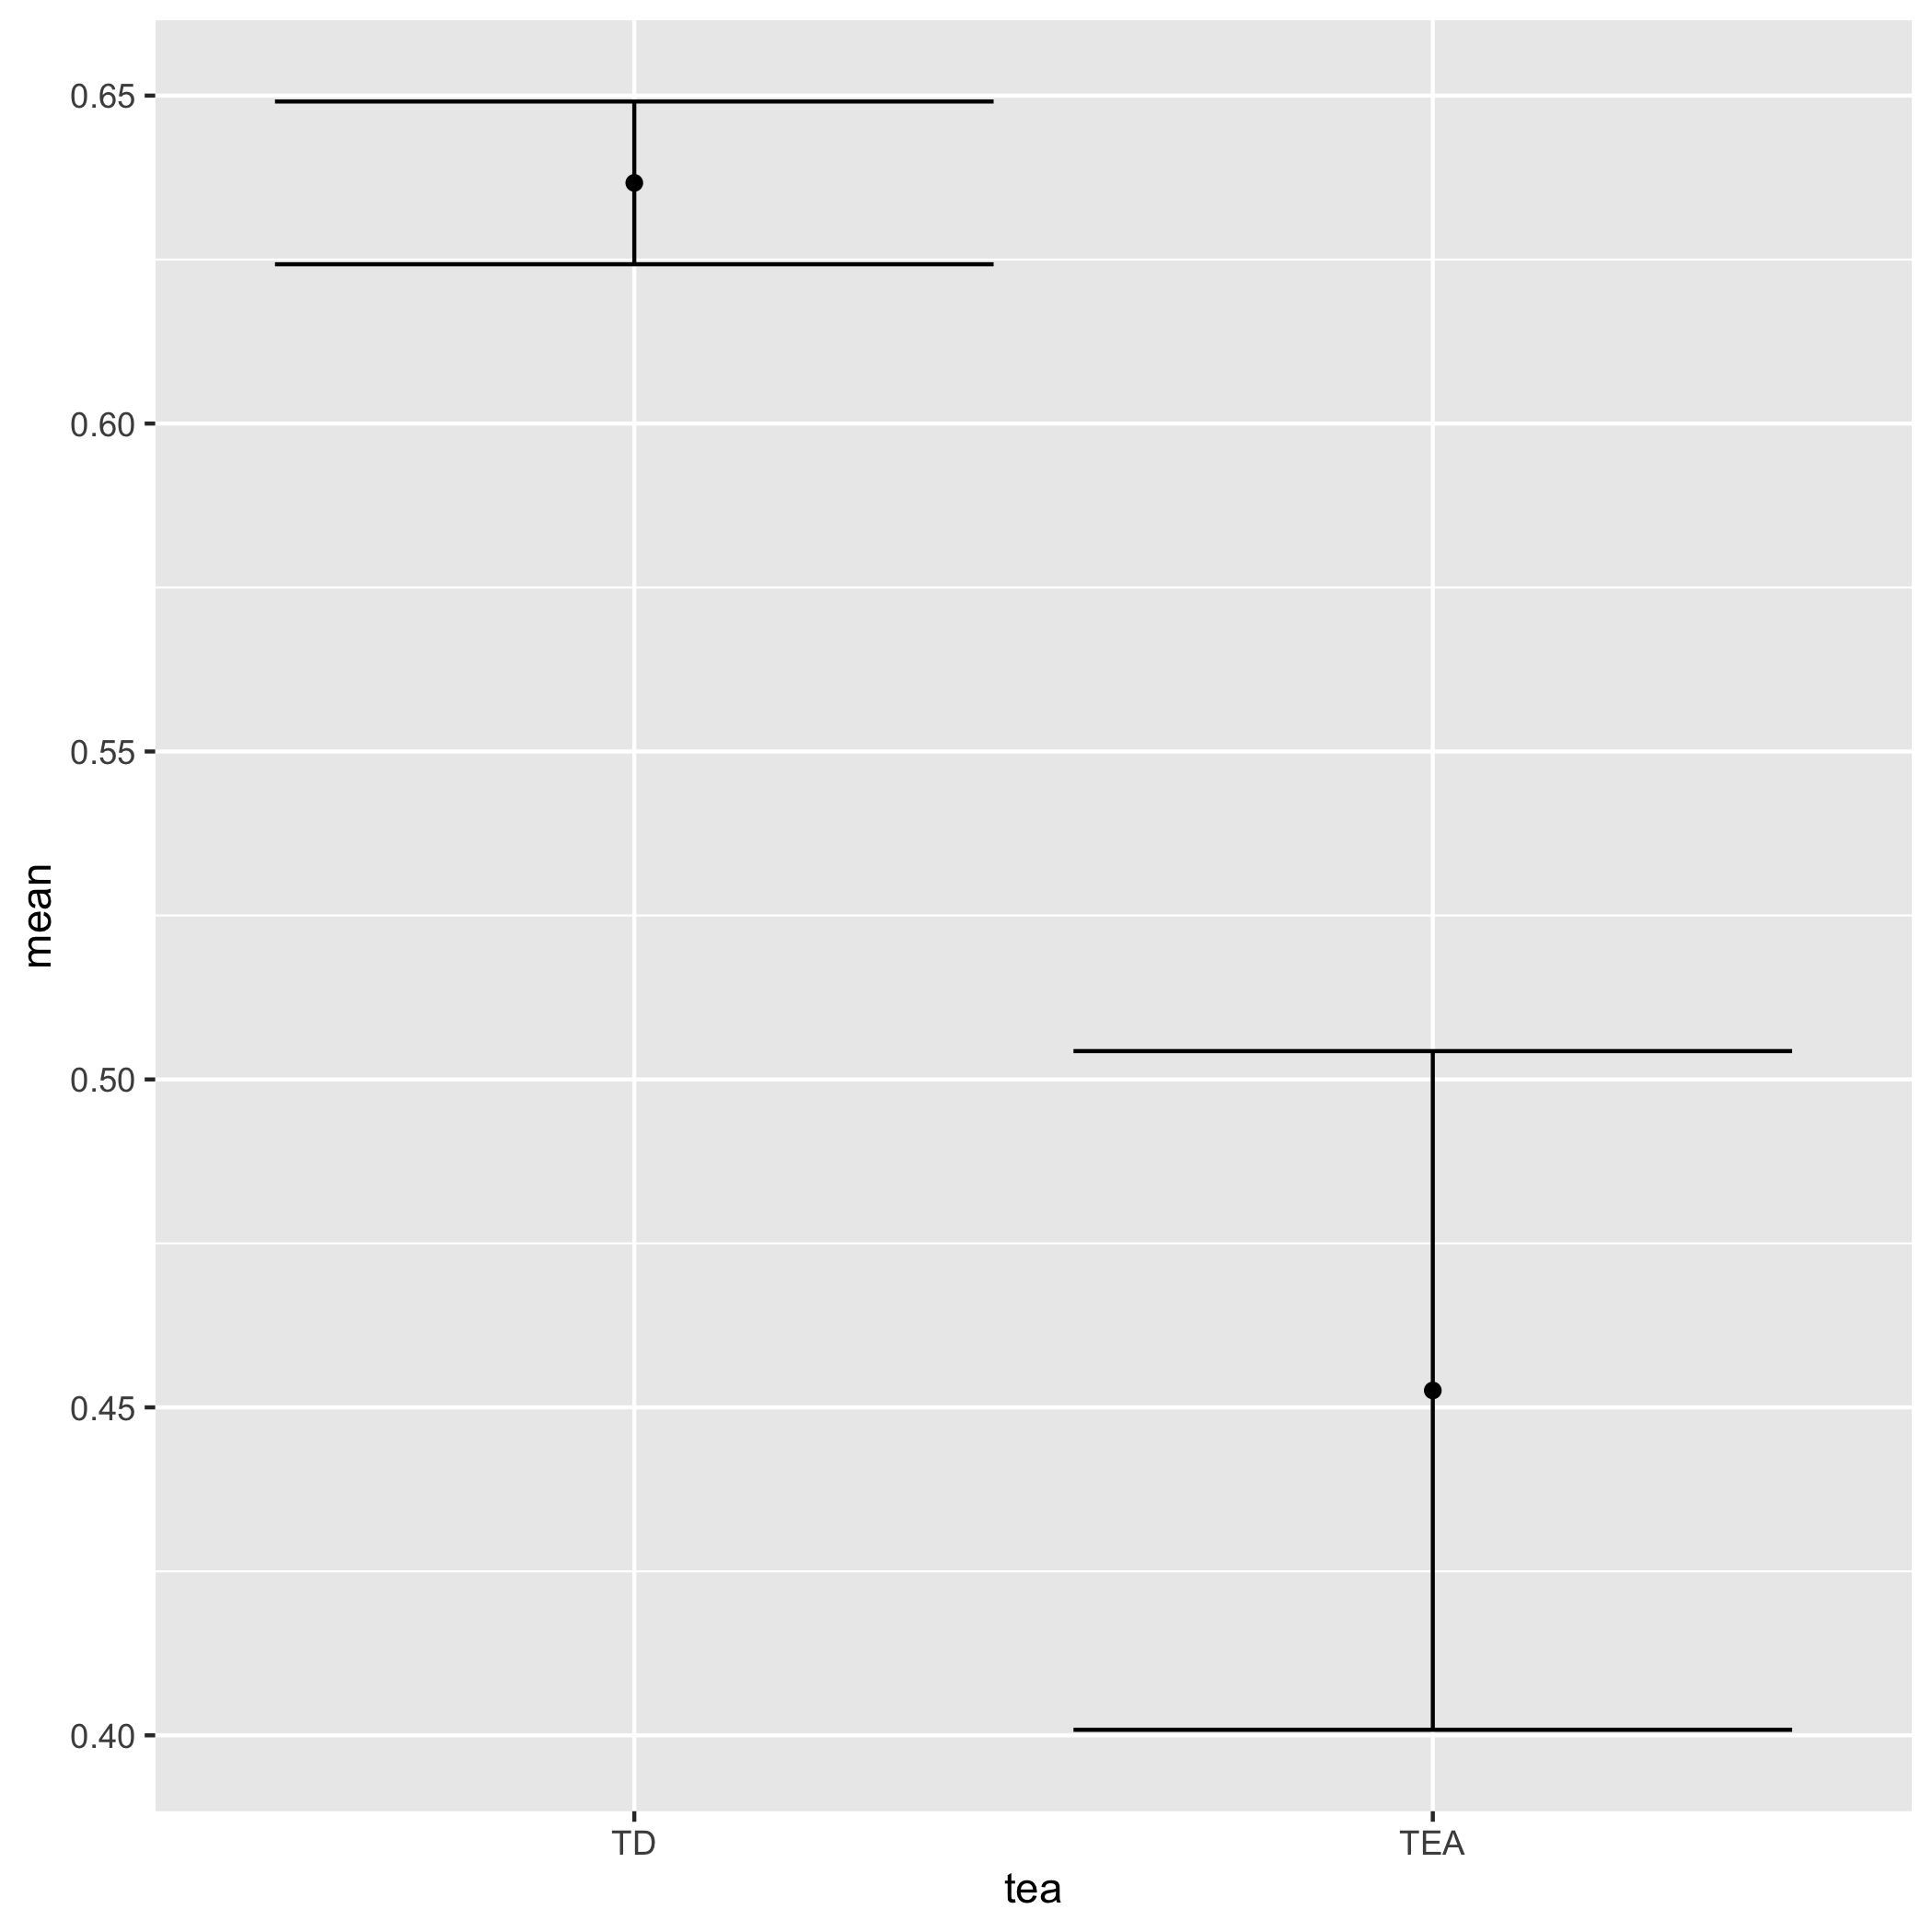
\includegraphics[scale=0.2]{./teaMainAlternancia.png}}
  \centering
\end{figure}

\begin{figure}[H]
  \caption{Visualizing effect of variable}
  \noindent\makebox[\textwidth]{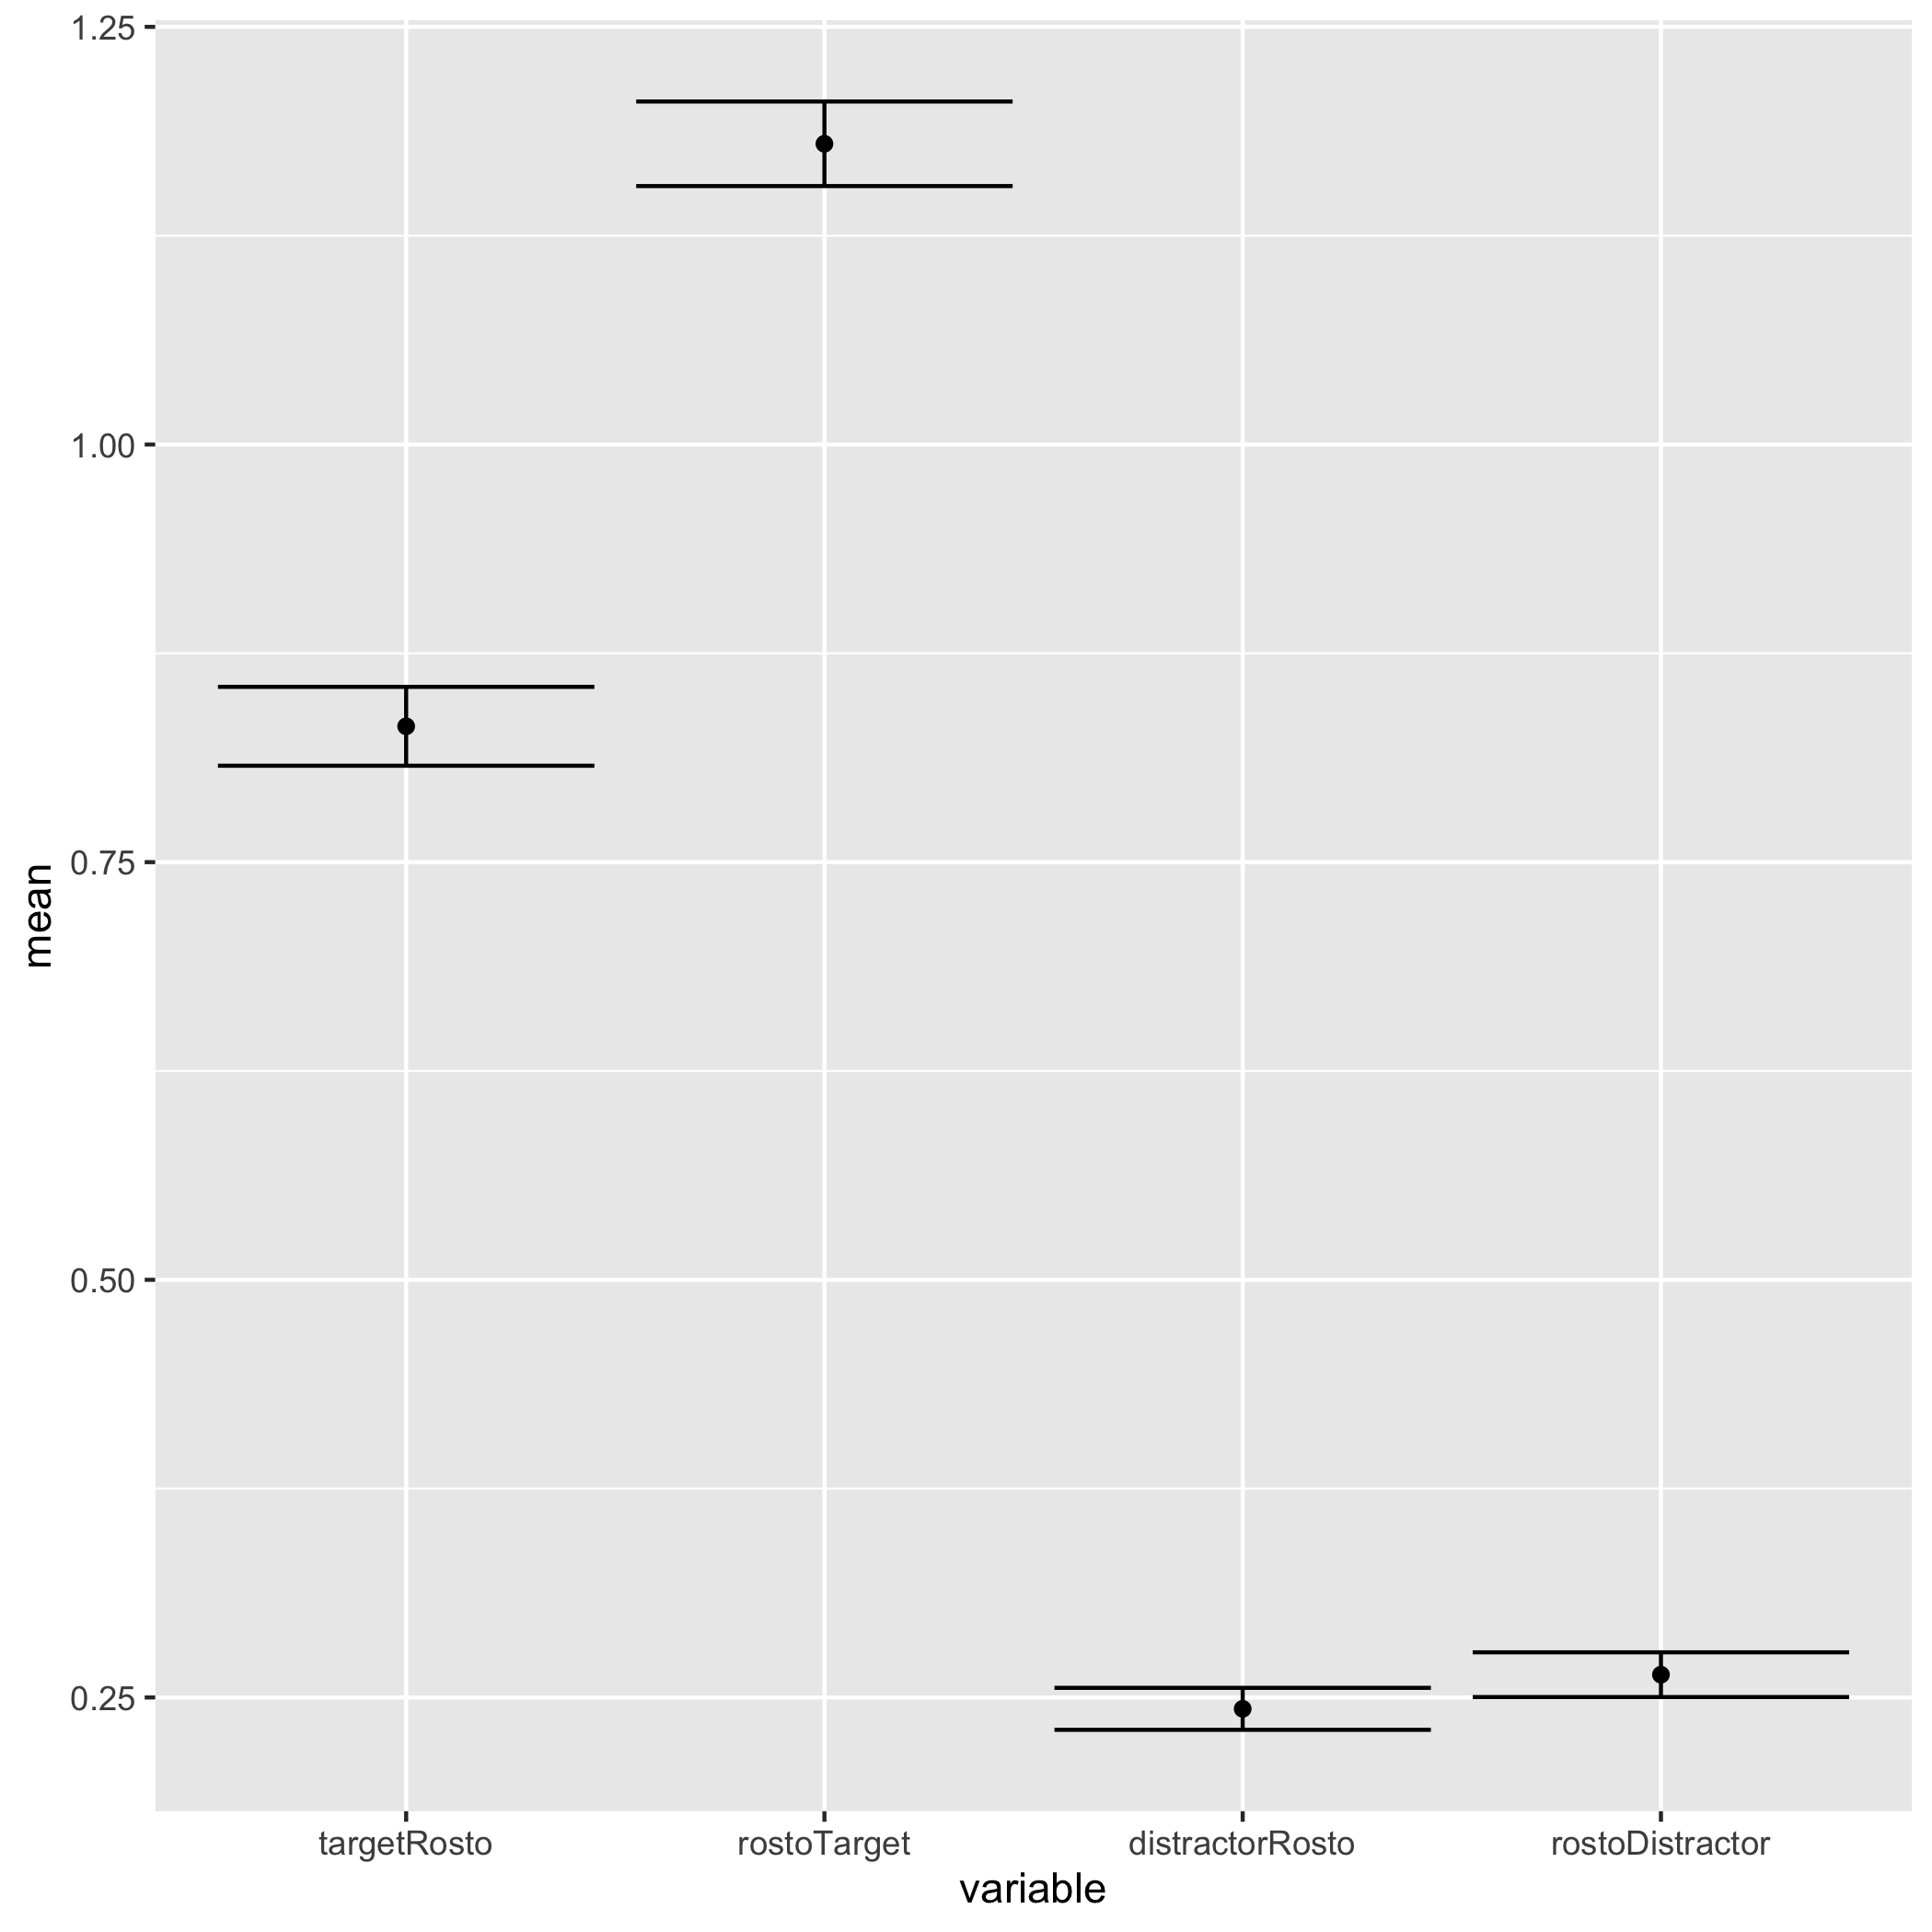
\includegraphics[scale=0.2]{./variableAlternancia.png}}
  \centering
\end{figure}

\begin{figure}[H]
  \caption{Visualizing effect of condition}
  \noindent\makebox[\textwidth]{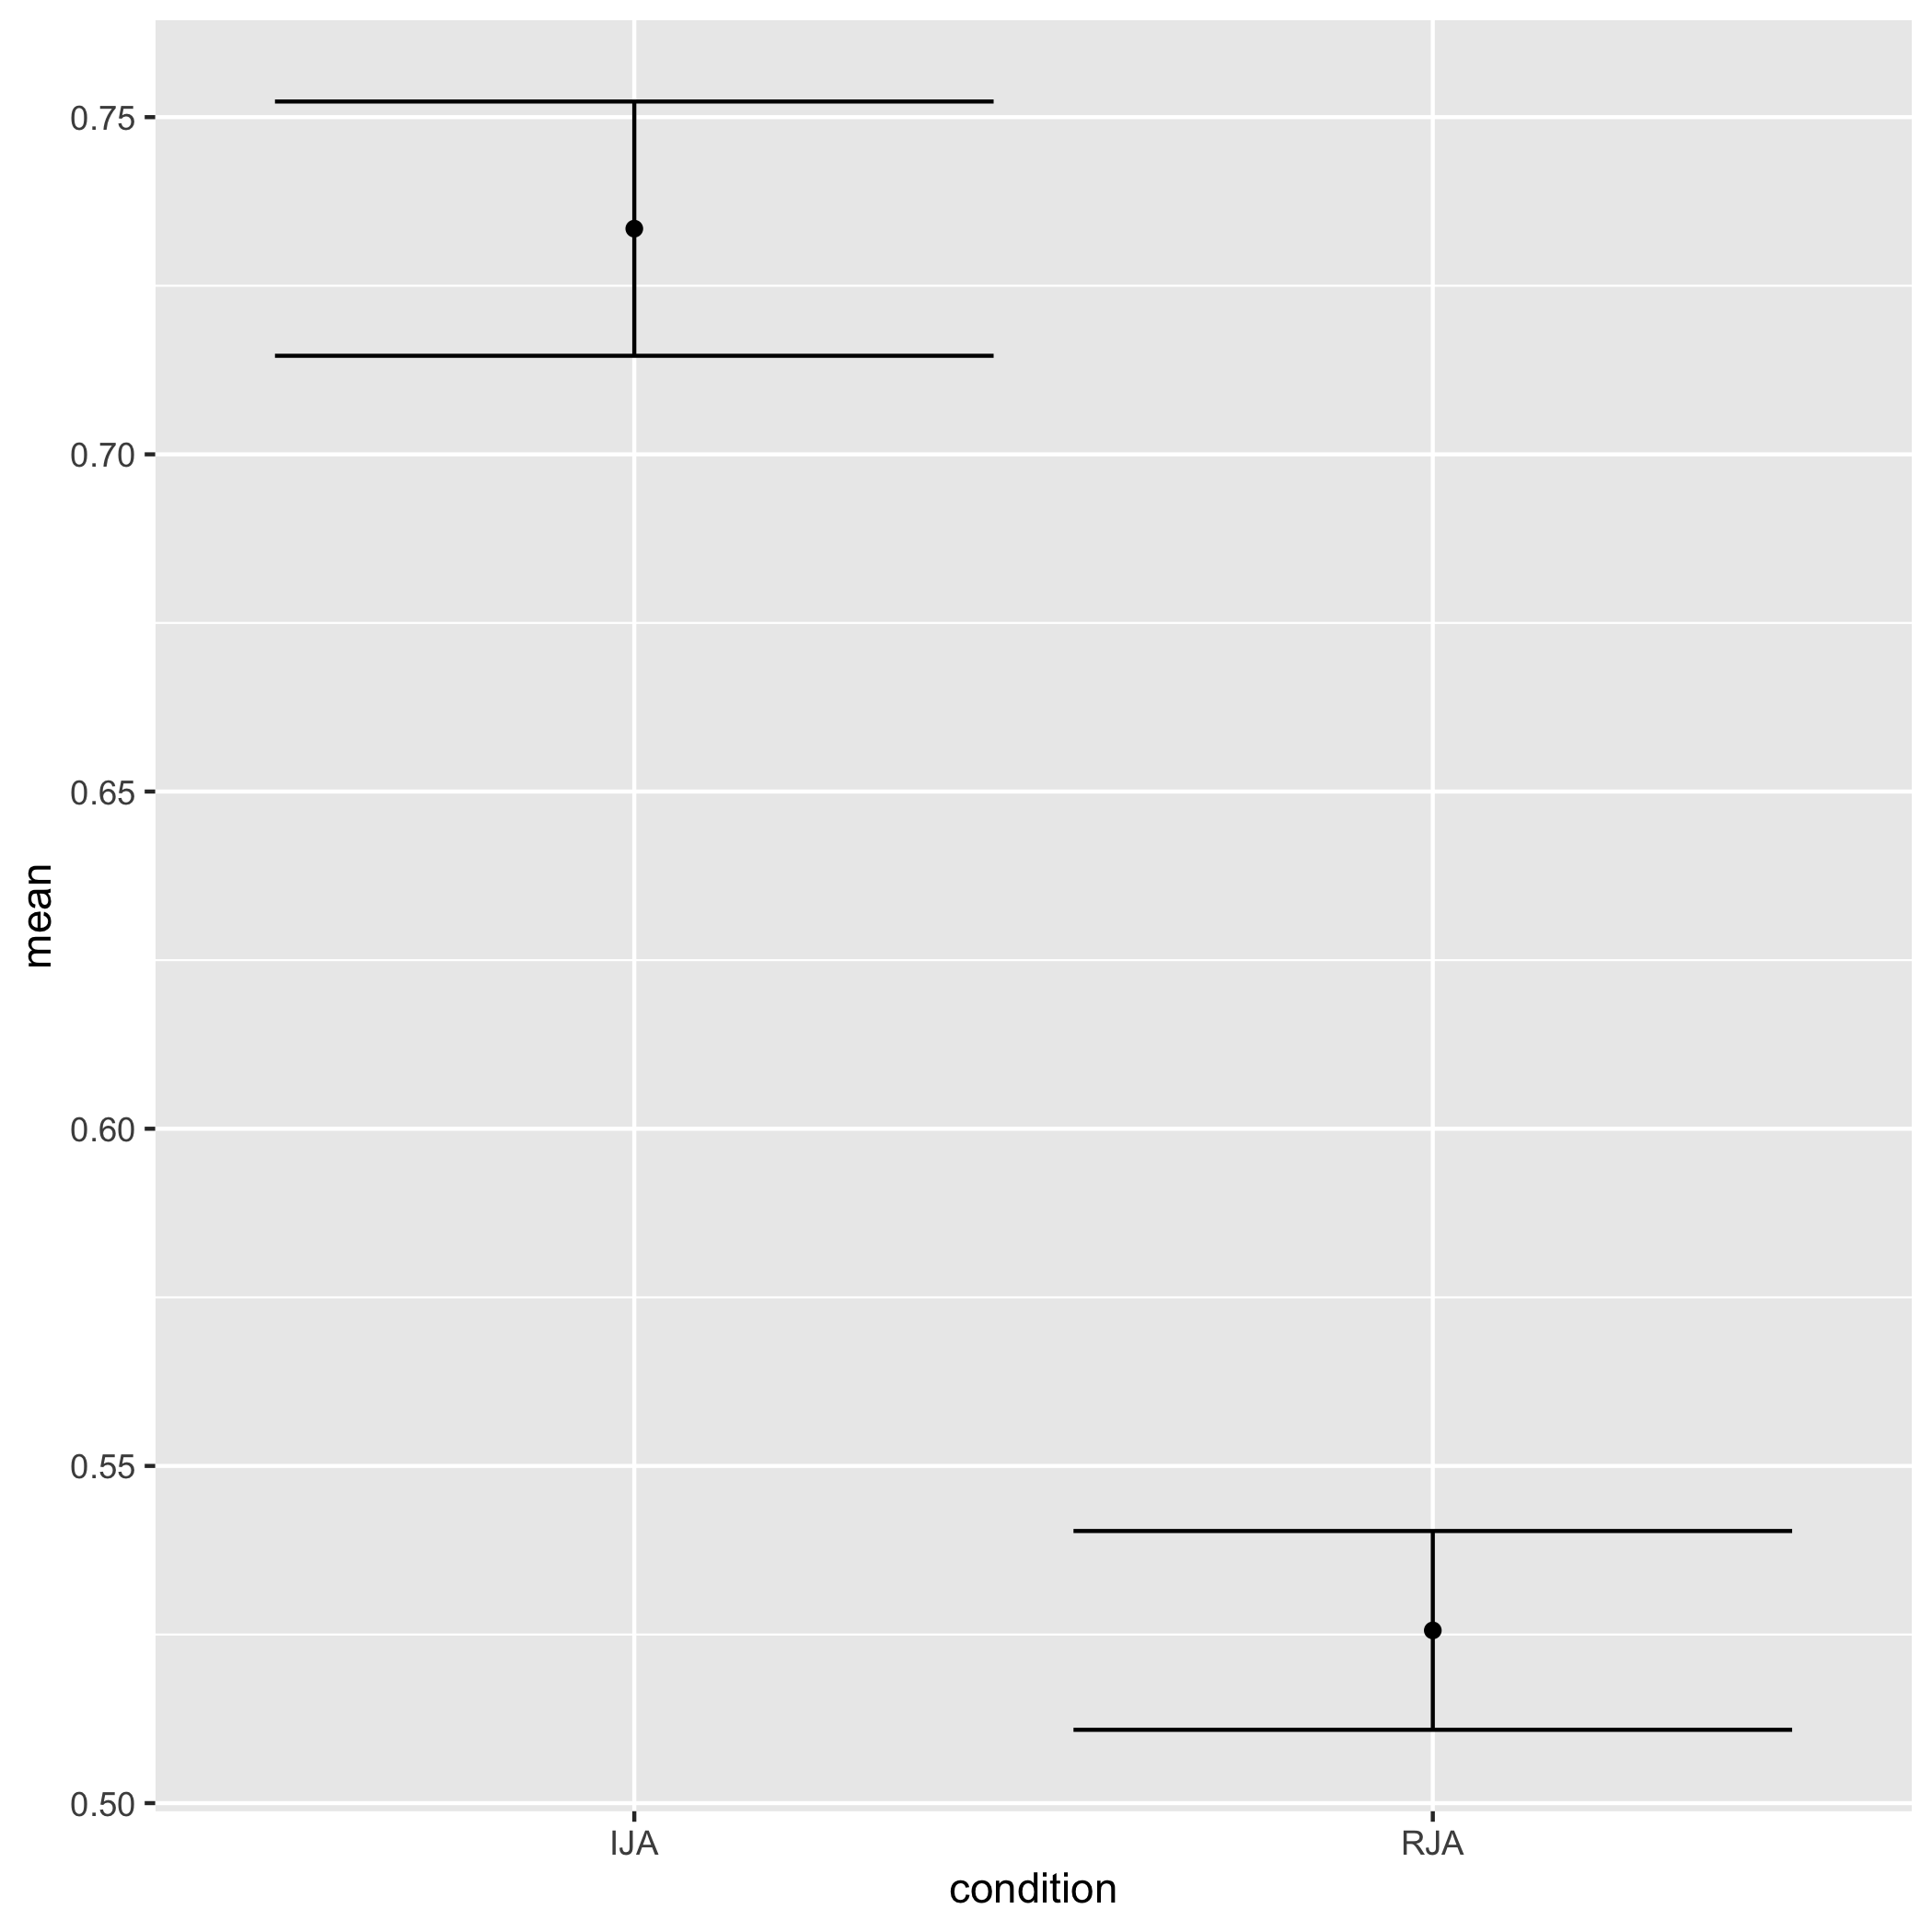
\includegraphics[scale=0.2]{./conditionAlternancia.png}}
  \centering
\end{figure}

\begin{figure}[H]
  \caption{Visualizing interaction of condition and variable}
  \noindent\makebox[\textwidth]{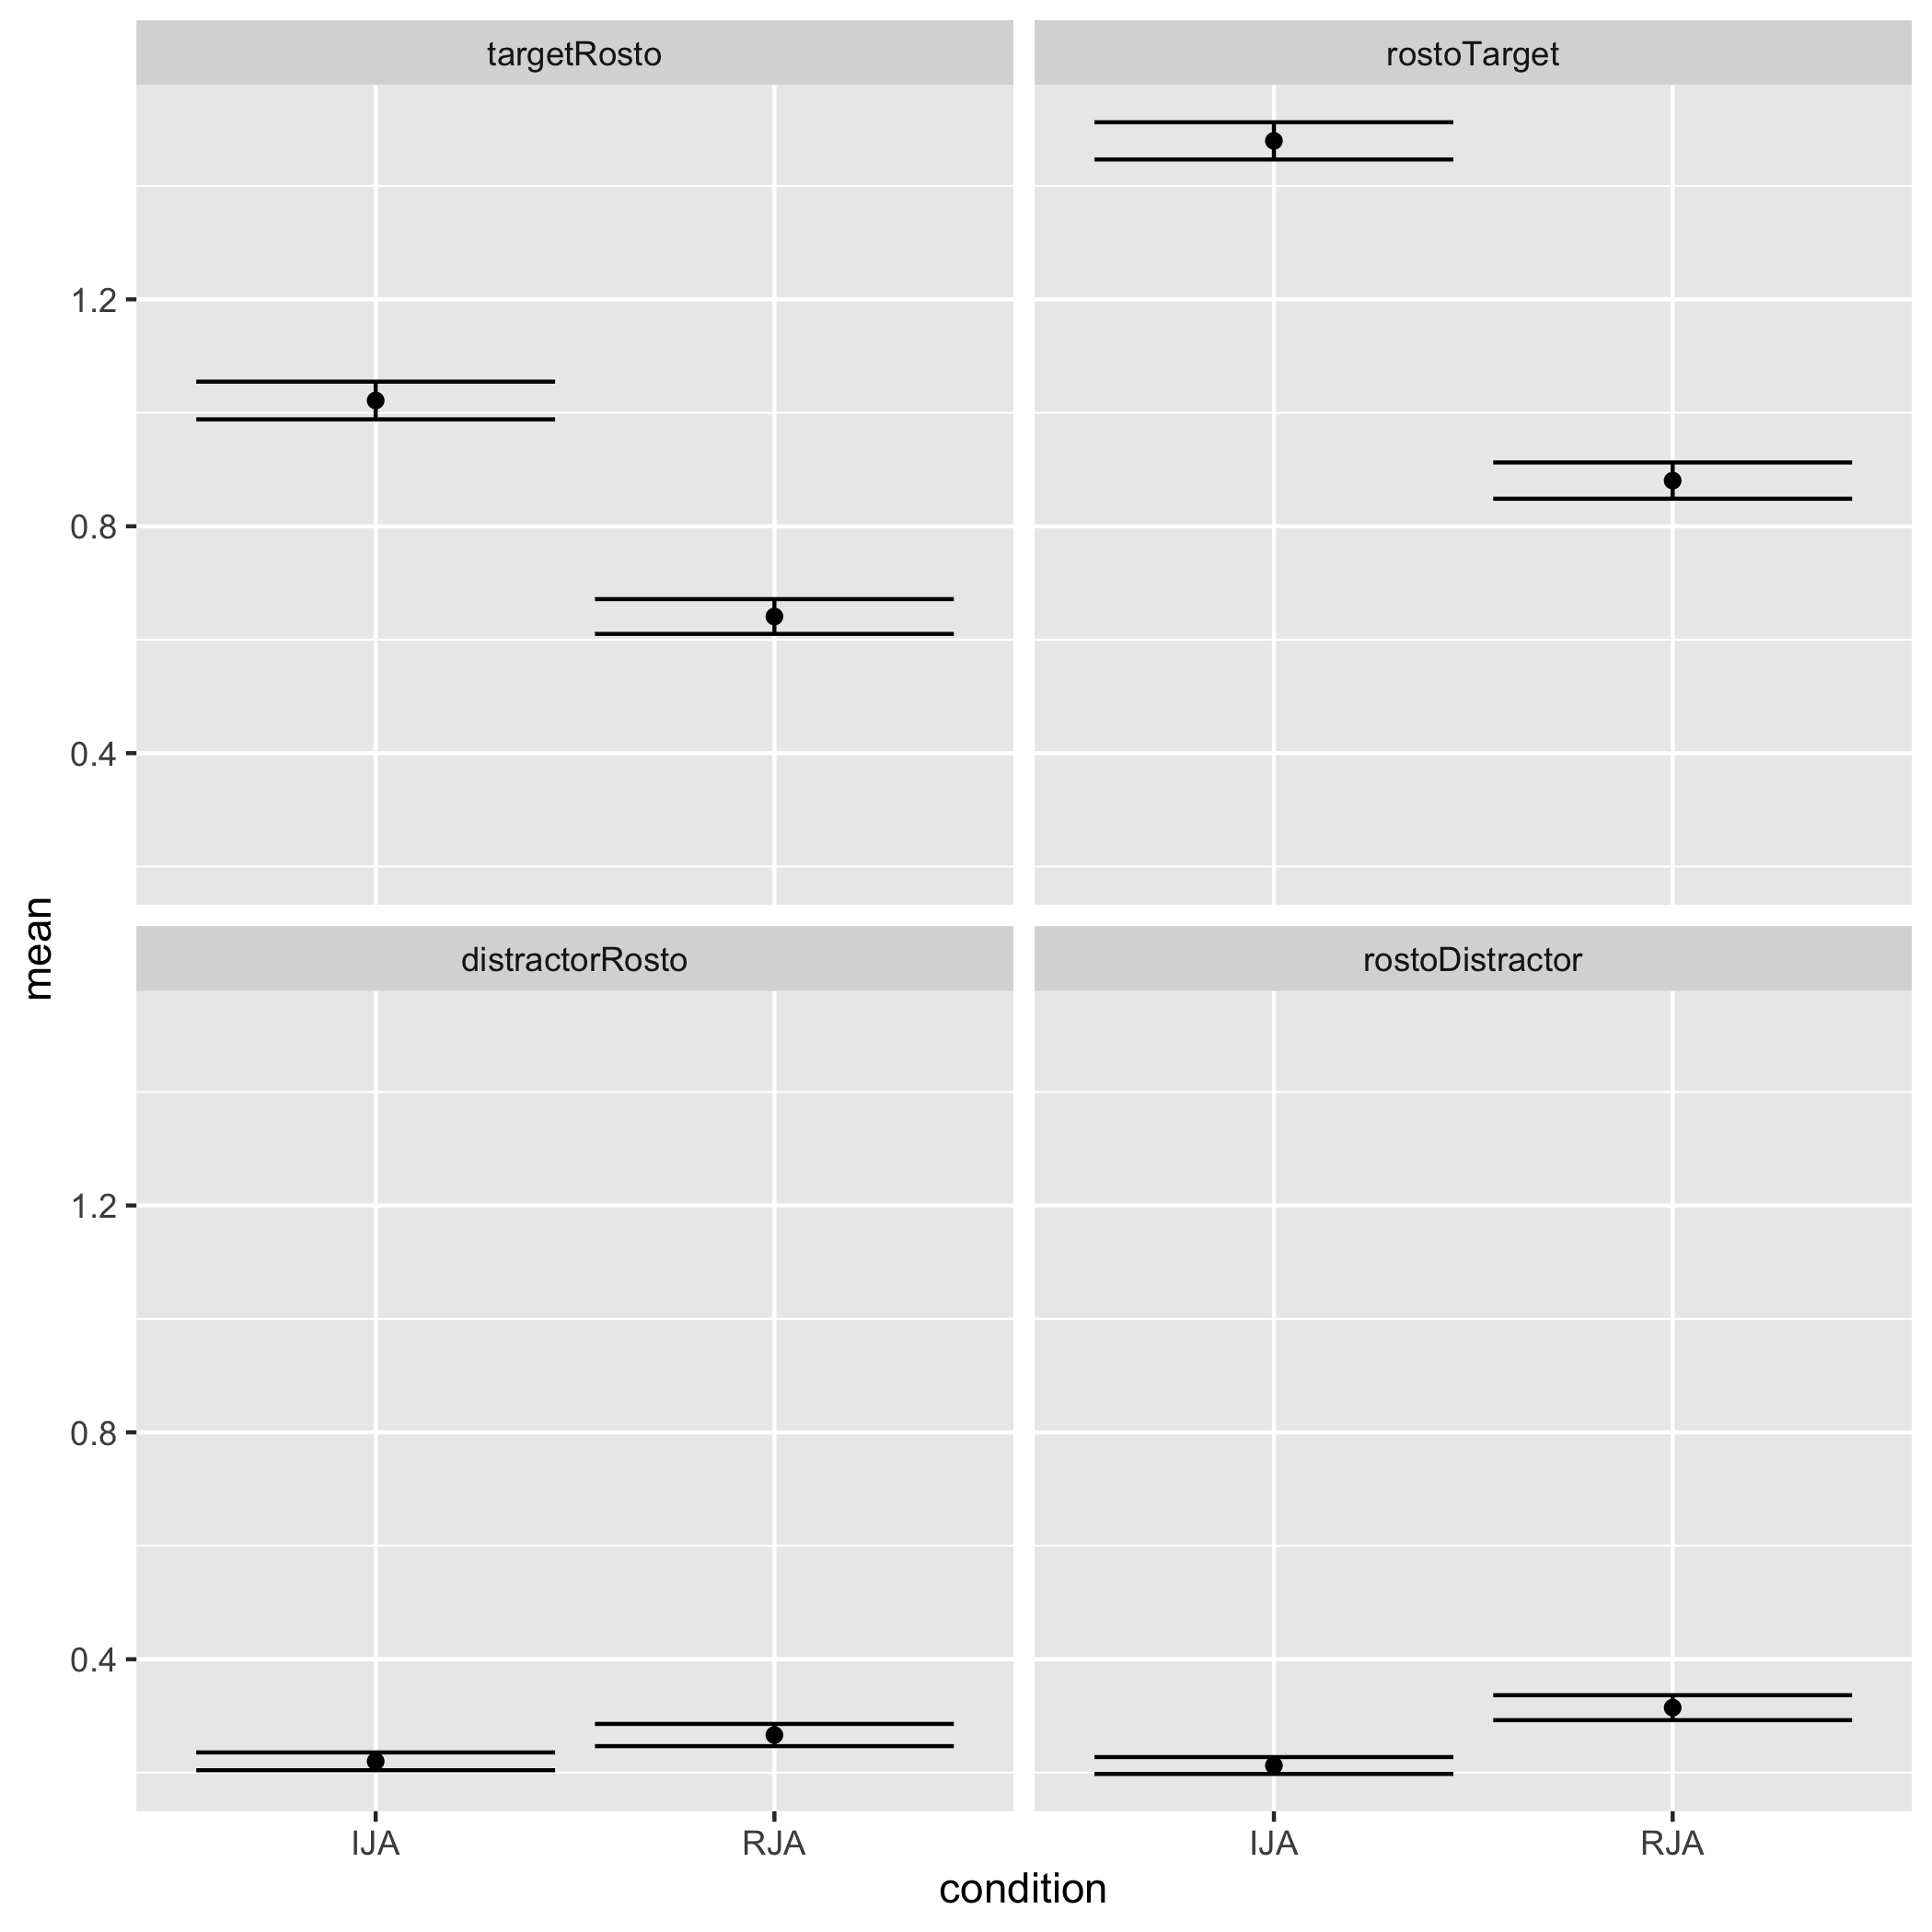
\includegraphics[scale=0.2]{./conditionVariableAlternancia.png}}
  \centering
\end{figure}

\begin{figure}[H]
  \caption{Visualizing interaction between tea and variable}
  \noindent\makebox[\textwidth]{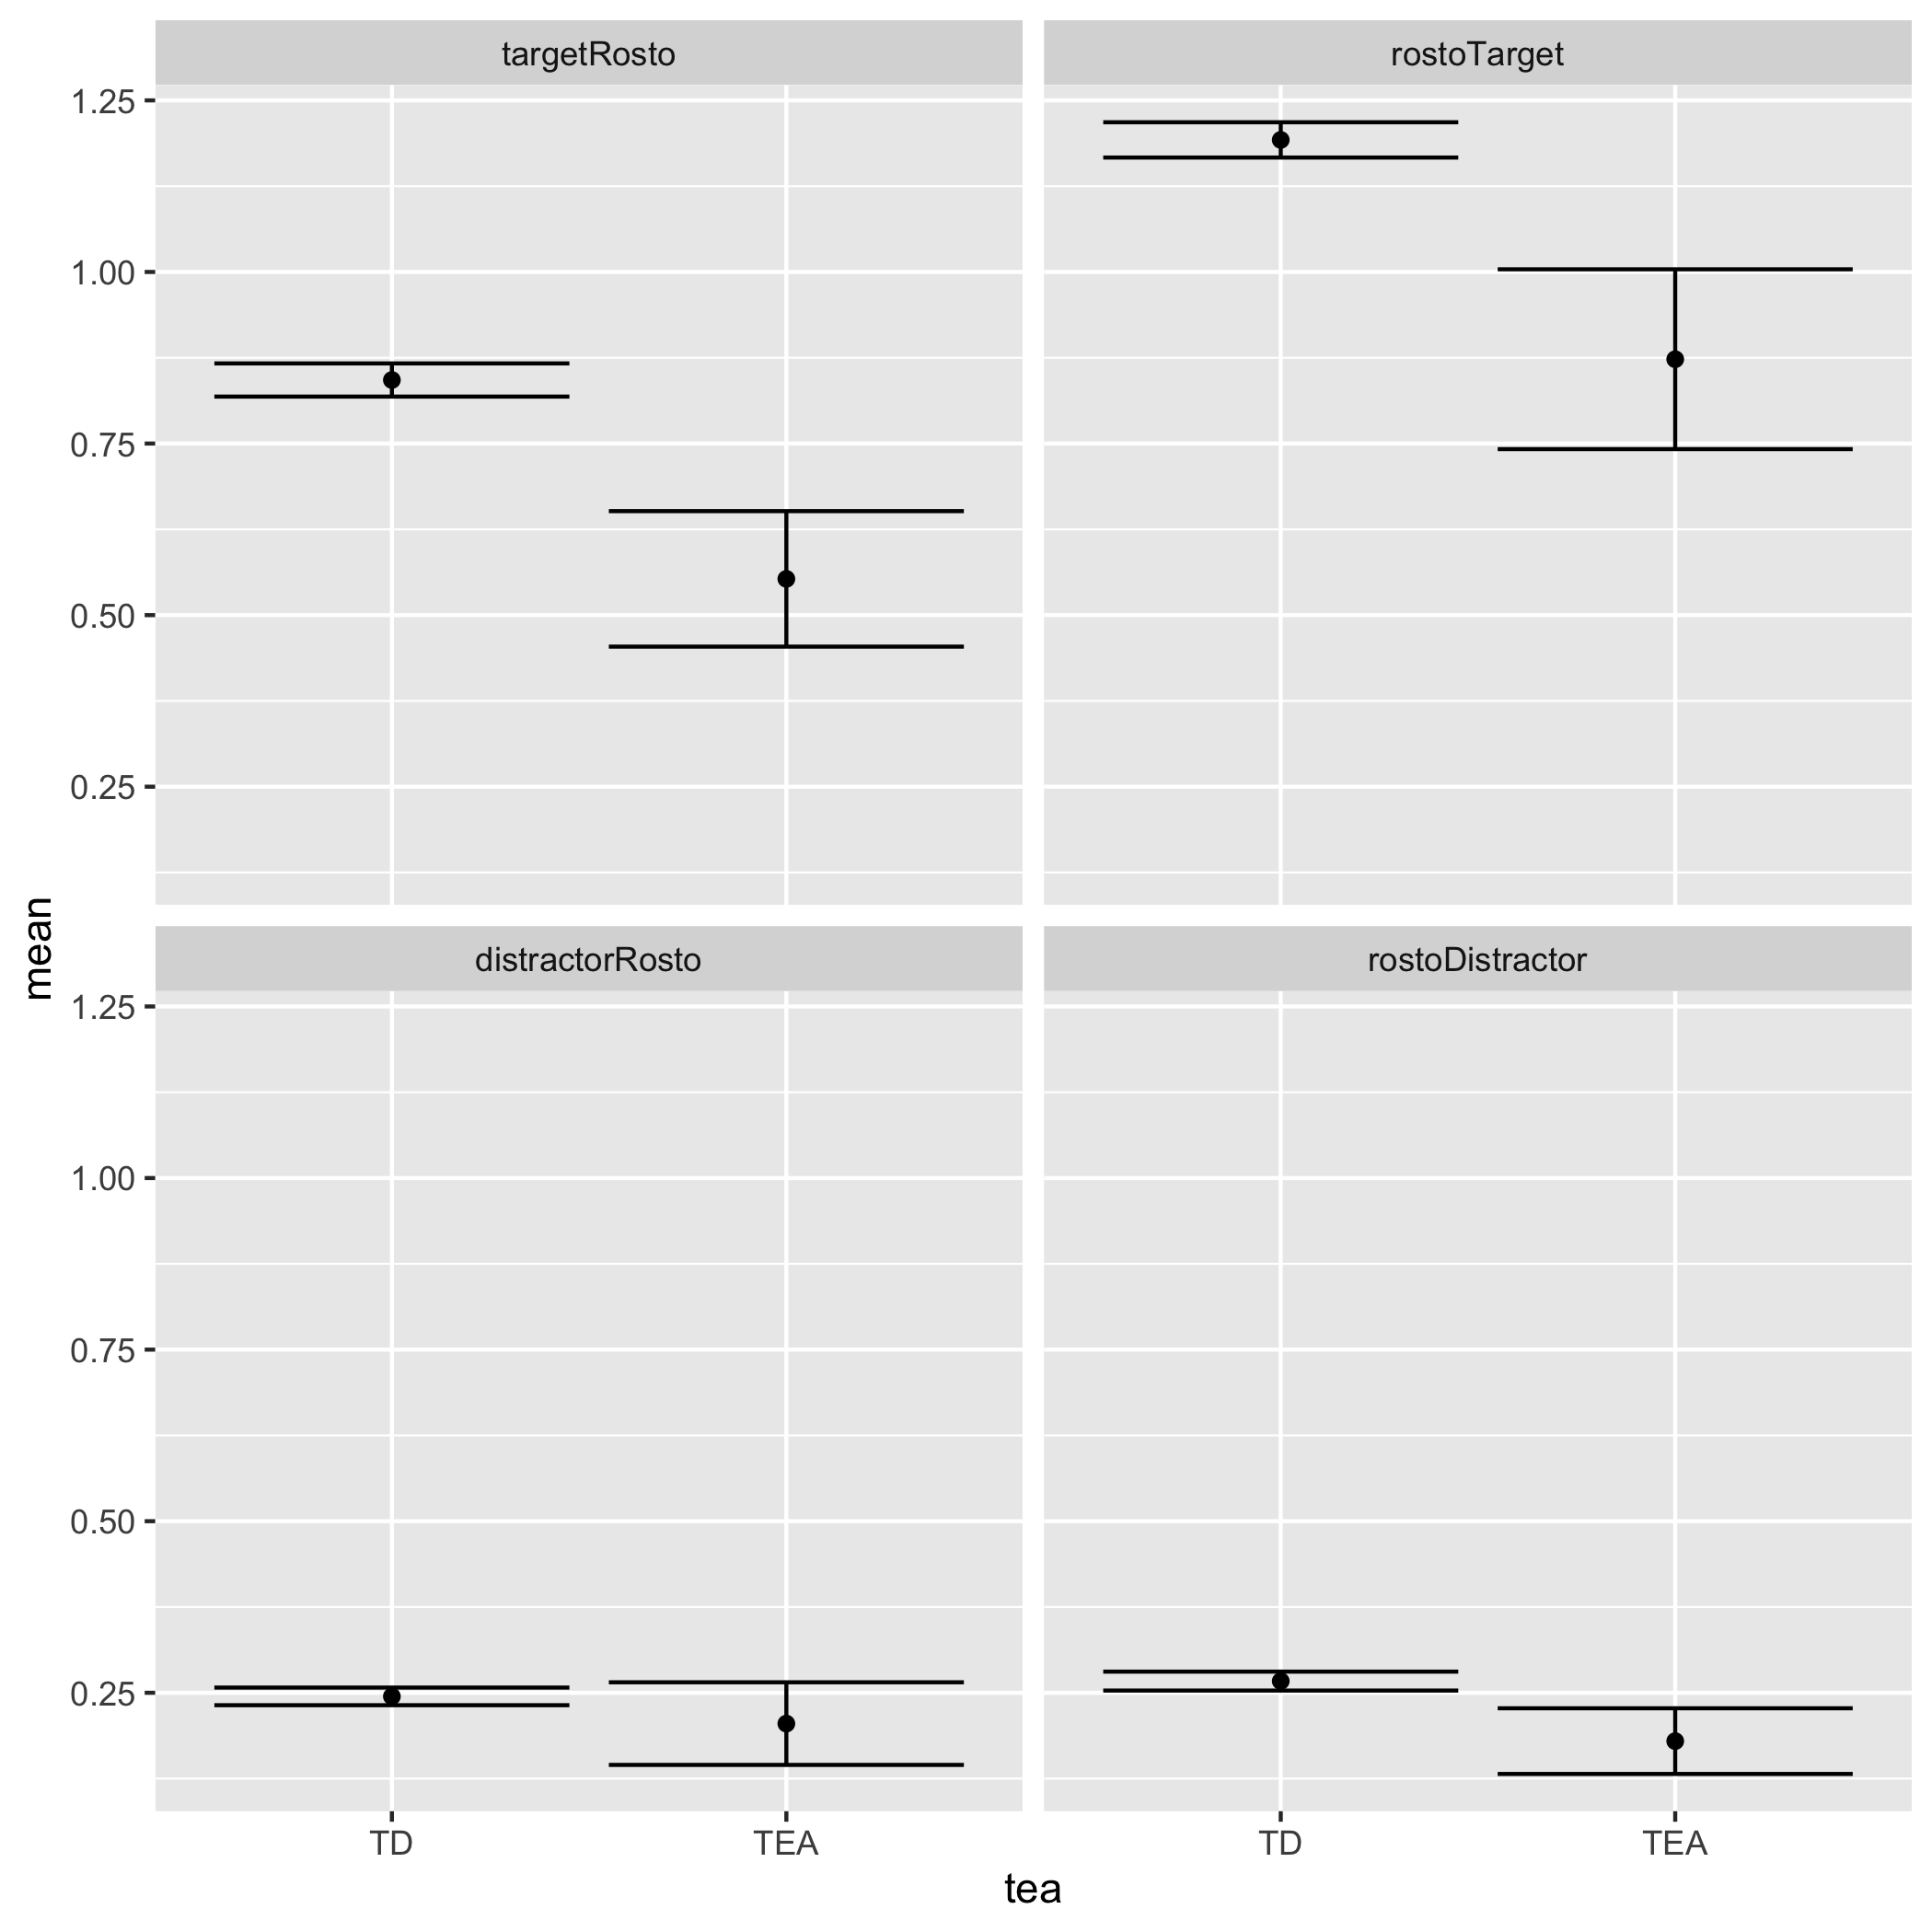
\includegraphics[scale=0.2]{./teaVariableAlternancia.png}}
  \centering
\end{figure}


\subsection{Proporção}

\begin{table}[ht]
\centering
\begin{tabular}{lrrrrr}
  \hline
 & Df & Sum Sq & Mean Sq & F value & Pr($>
$F) \\ 
  \hline
condition              & 1 & 0.00 & 0.00 &
 0.00 & 1.0000 \\ 
  tea                    & 1 & 0.00 & 0.00
 & 0.00 & 1.0000 \\ 
  variable               & 3 & 101.30 & 33
.77 & 1452.10 & 0.0000 \\ 
  condition:tea          & 1 & 0.00 & 0.00
 & 0.00 & 1.0000 \\ 
  condition:variable     & 3 & 20.65 & 6.8
8 & 295.96 & 0.0000 \\ 
  tea:variable           & 3 & 0.35 & 0.12
 & 5.01 & 0.0018 \\ 
  condition:tea:variable & 3 & 0.11 & 0.04
 & 1.62 & 0.1832 \\ 
  Residuals              & 3072 & 71.43 & 
0.02 &  &  \\ 
   \hline
\end{tabular}
\end{table}



\begin{figure}[H]
  \caption{Visualizing variable effect}
  \noindent\makebox[\textwidth]{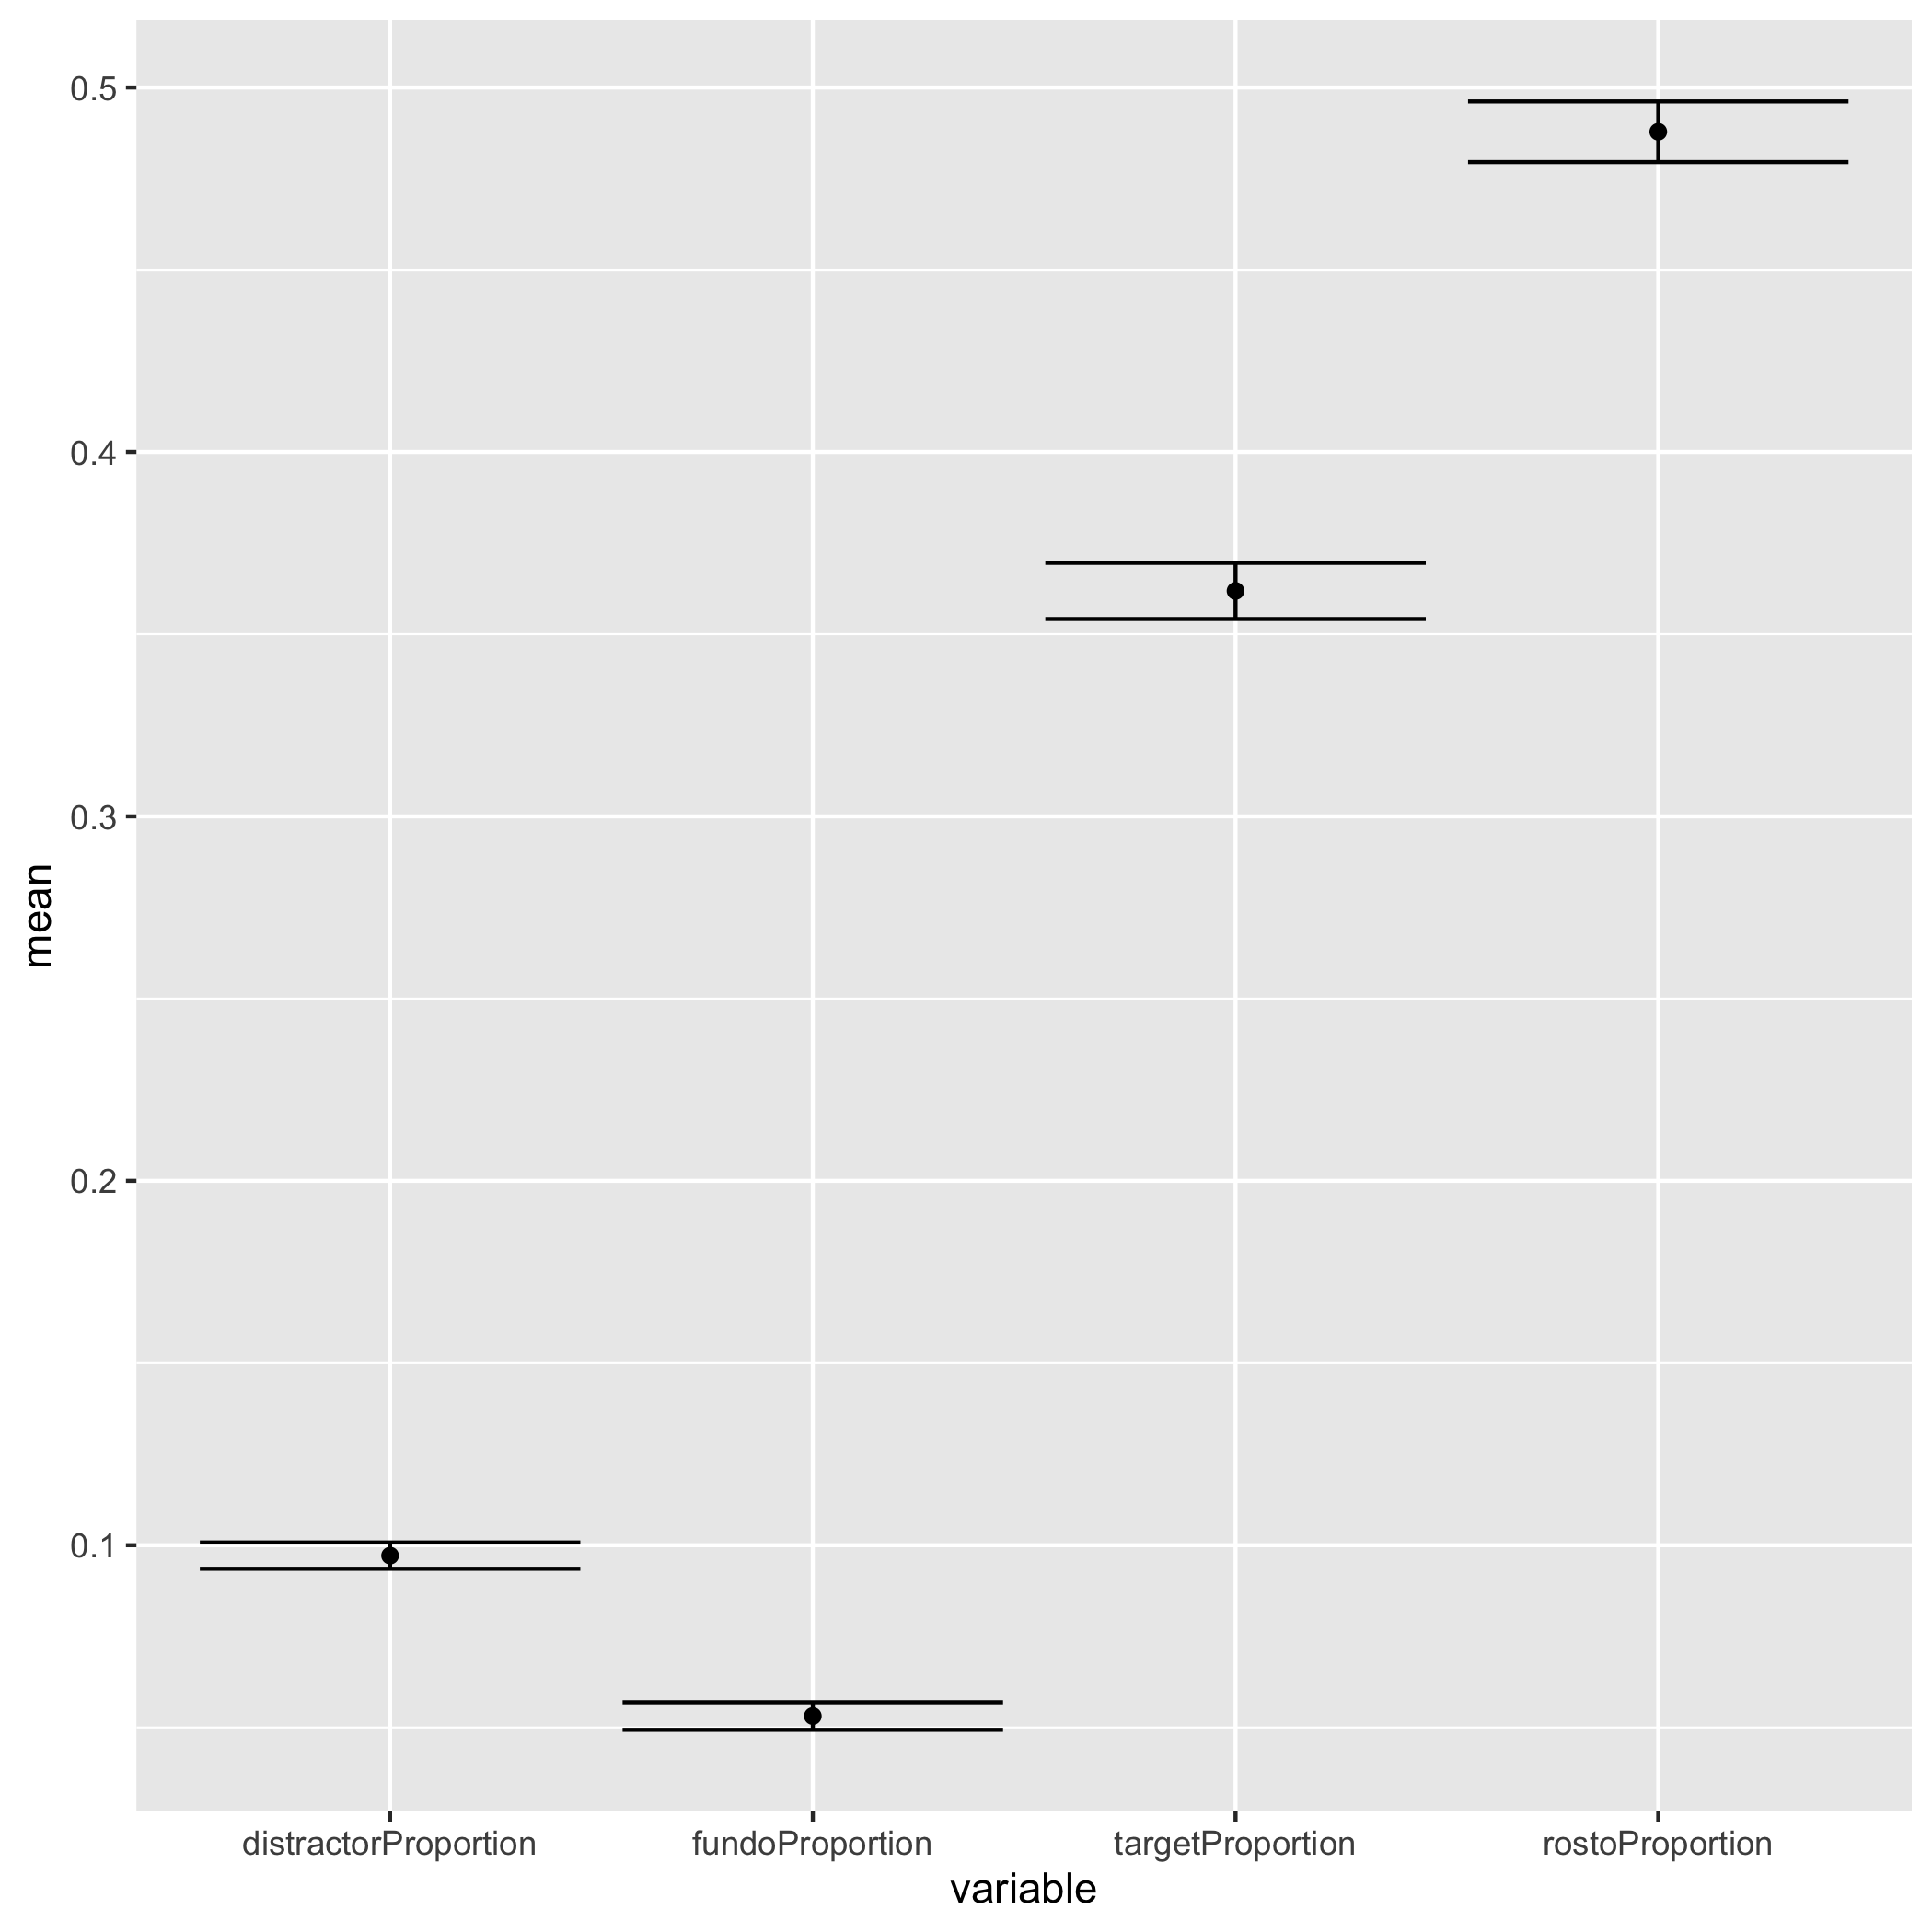
\includegraphics[scale=0.2]{./variableProportion.png}}
  \centering
\end{figure}

\begin{figure}[H]
  \caption{Visualizing interaction condition and variable}
  \noindent\makebox[\textwidth]{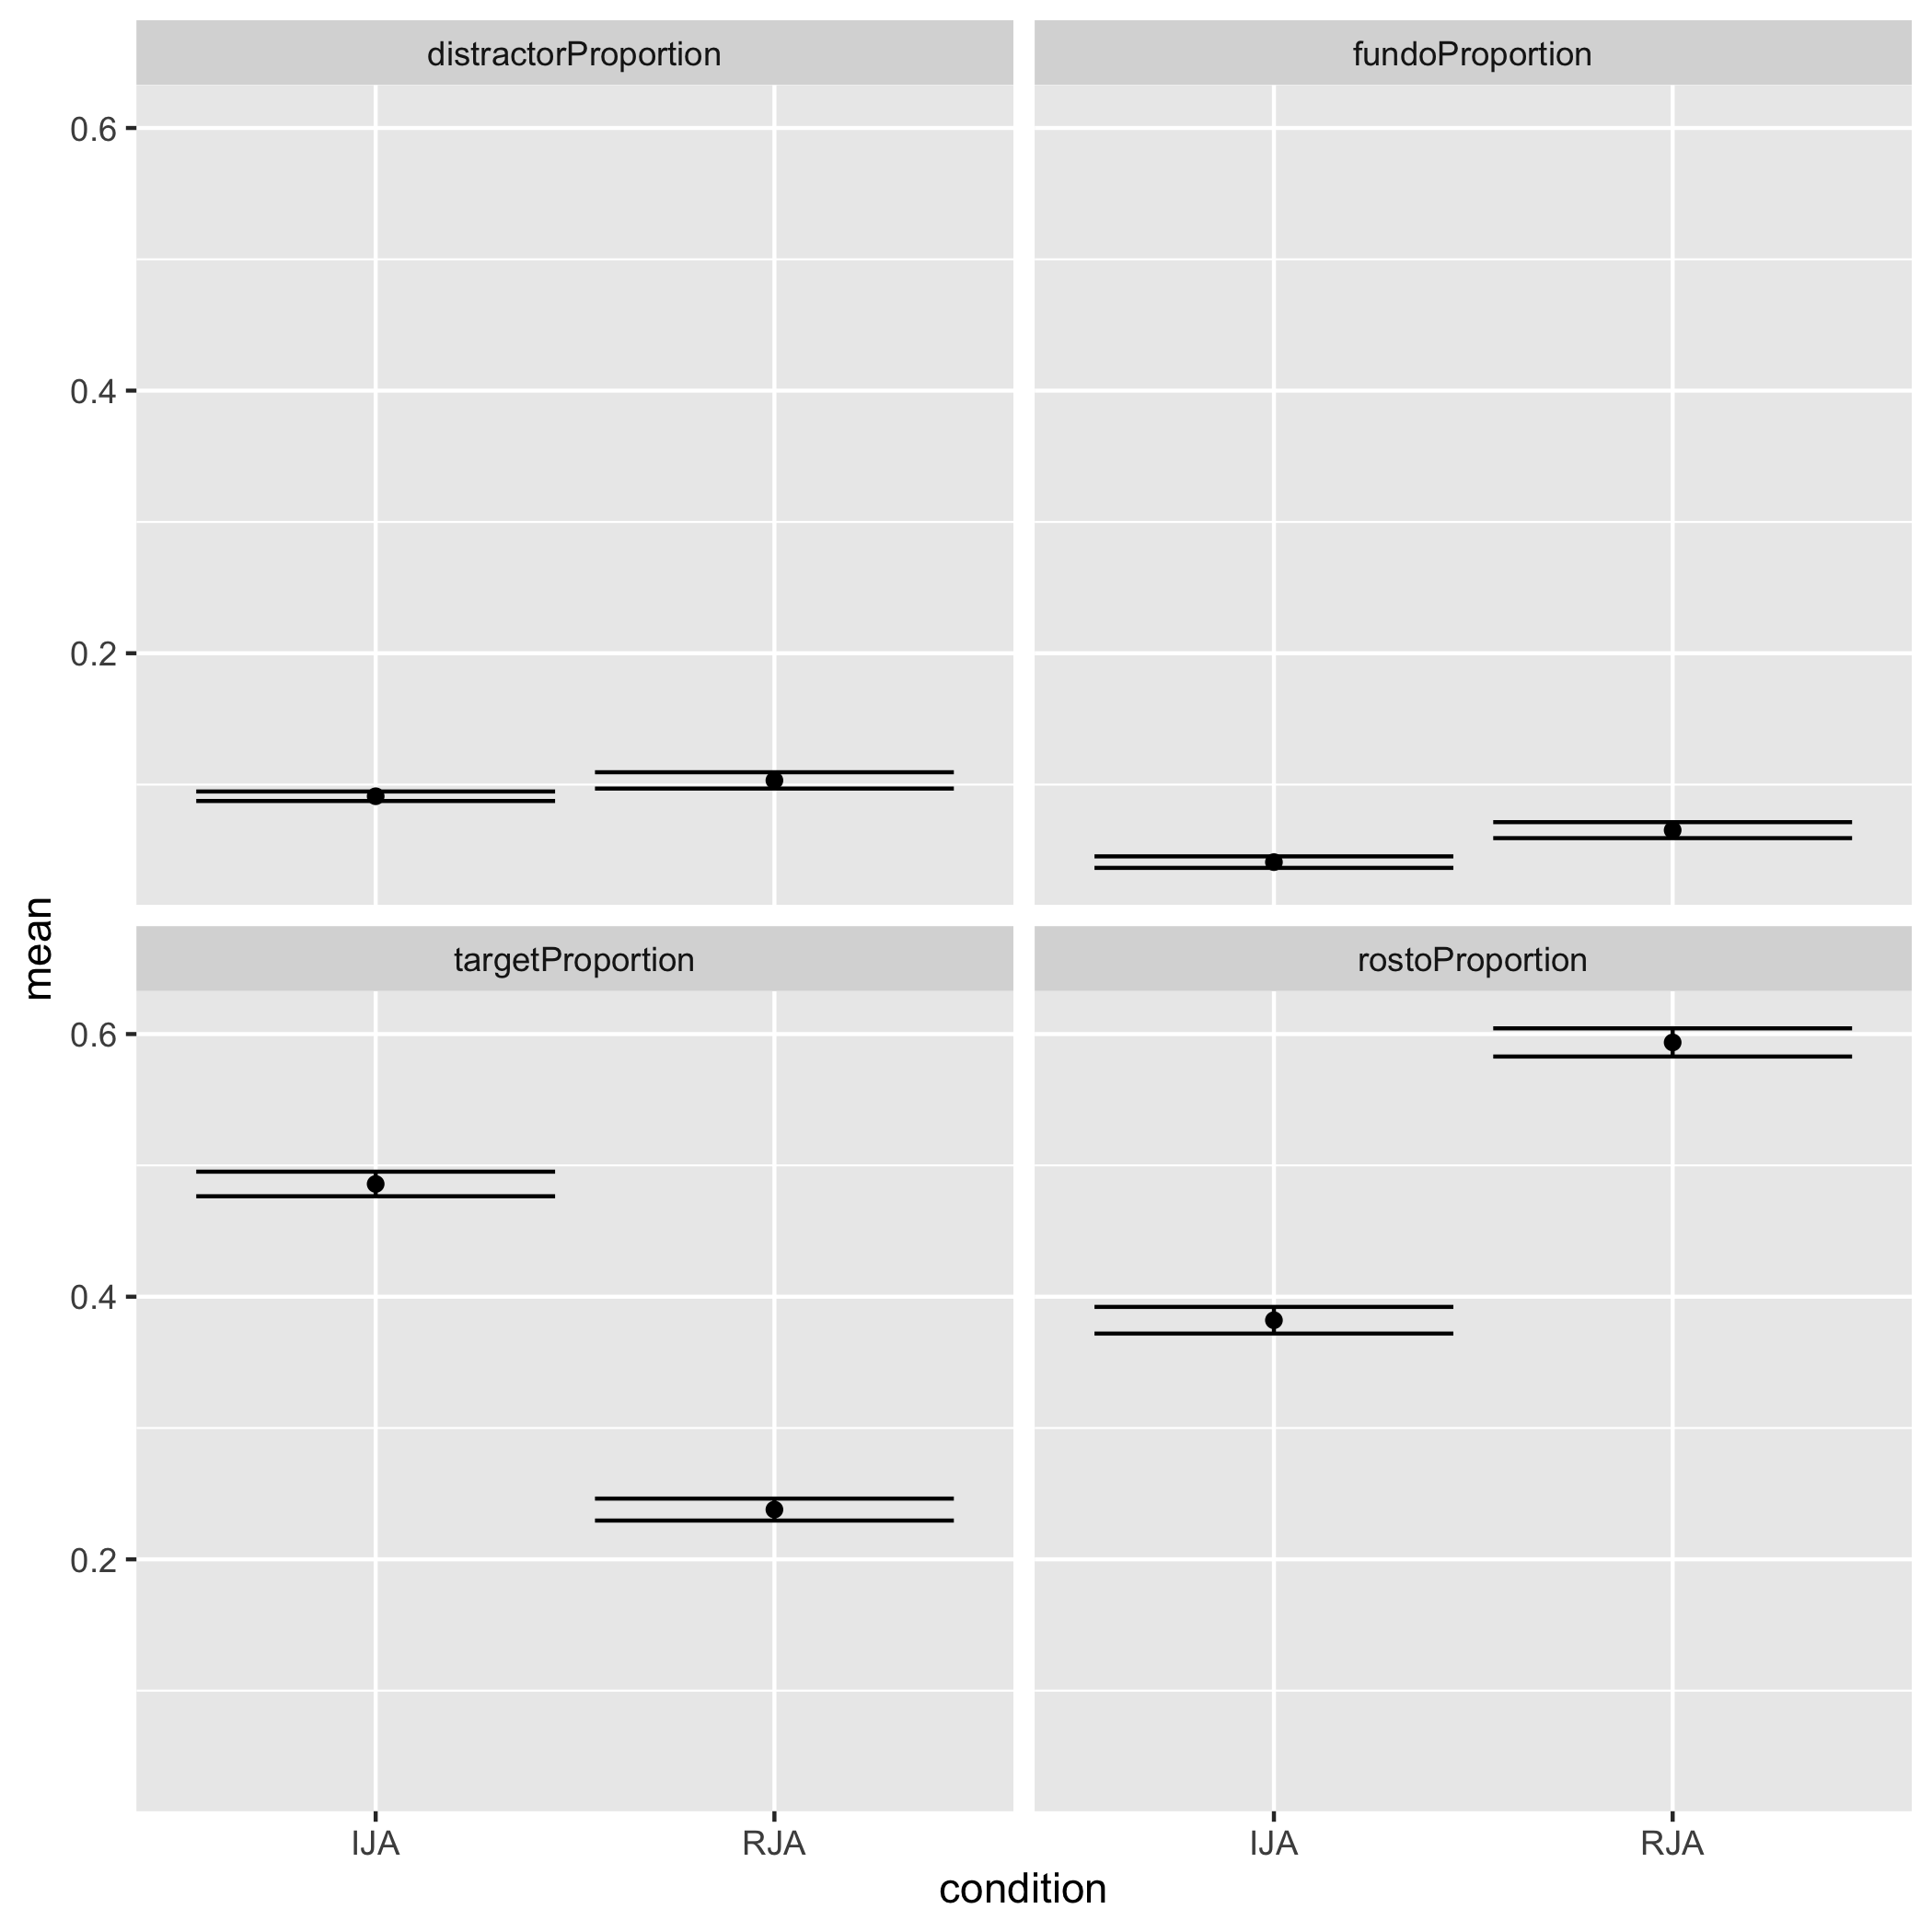
\includegraphics[scale=0.2]{./conditionVariableProportion.png}}
  \centering
\end{figure}

\begin{figure}[H]
  \caption{Visualizing interaction tea variable}
  \noindent\makebox[\textwidth]{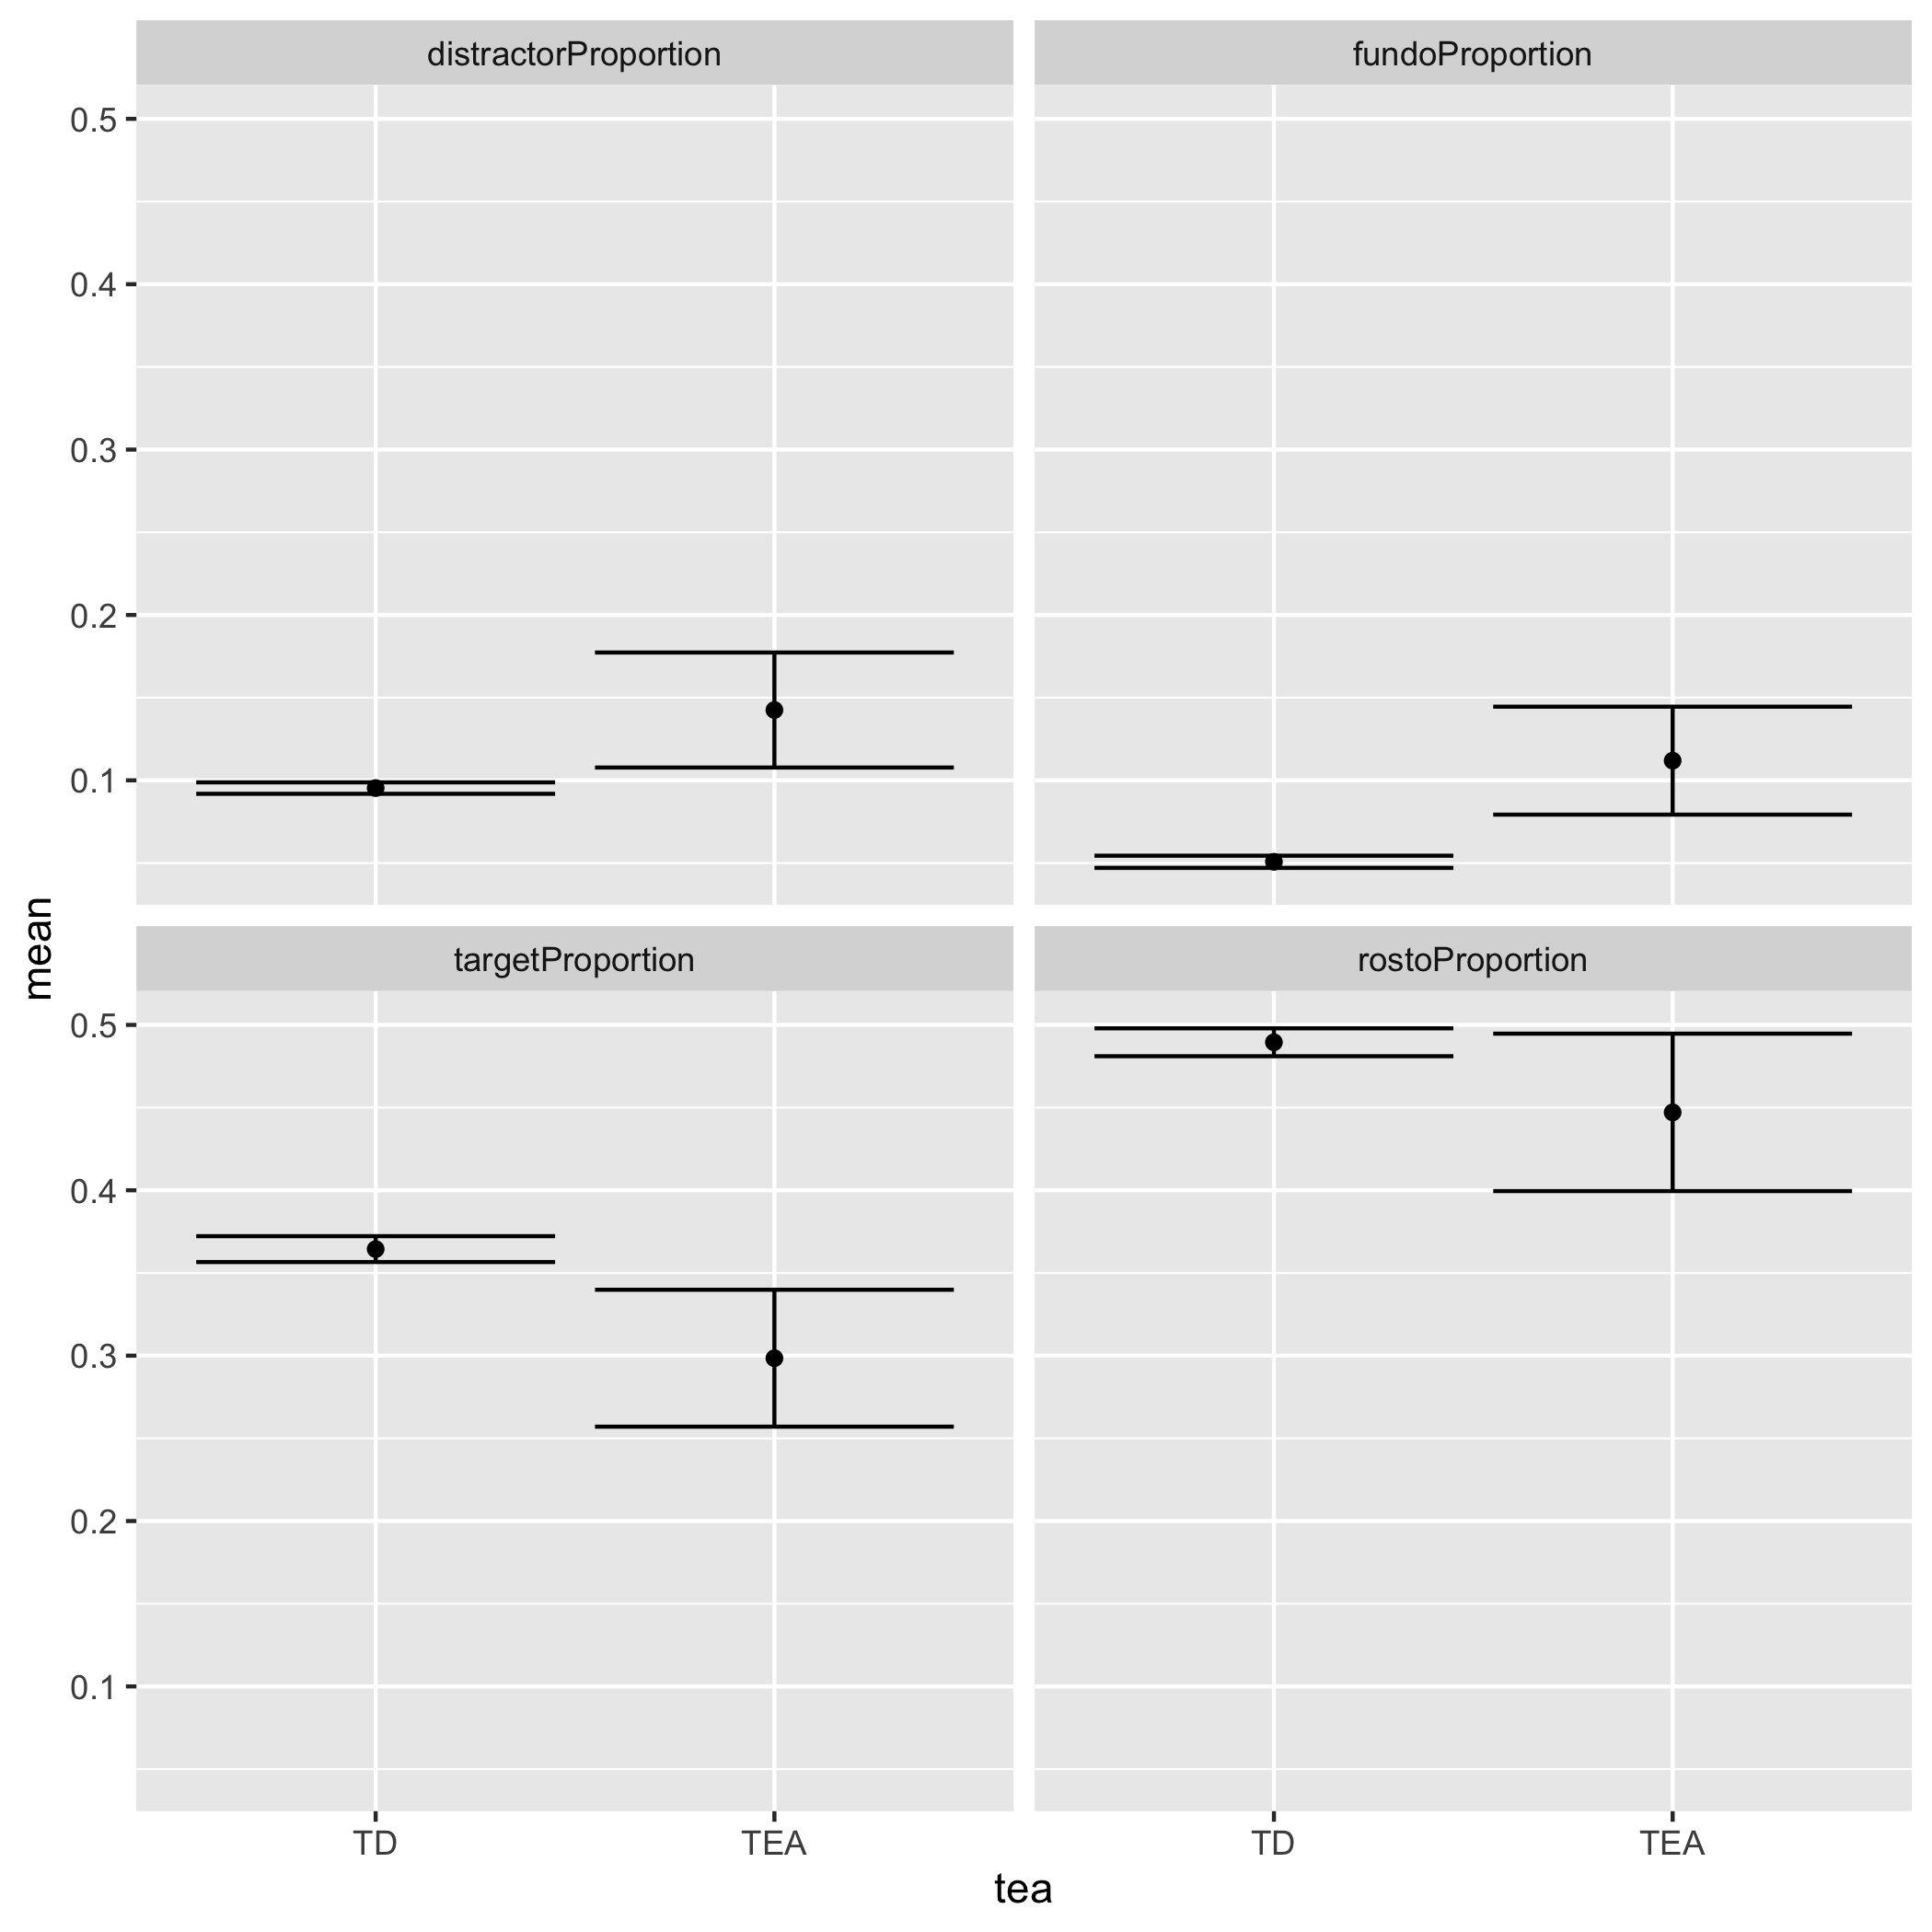
\includegraphics[scale=0.2]{./teaVariableProportion.png}}
  \centering
\end{figure}


\end{document}

